\section{Introduction}

\begin{singlespace} 
	\begin{quote}
		"[T]here is perhaps an over-emphasis of technology in [Leak Detection Systems]. A recurring theme is that of false alarms. The implication is that [a Leak Detection System] is expected to perform as an elementary industrial automation alarm, with an on/off state and six-sigma reliability. Any alarm that does not correspond to an actual leak is, with this thinking, an indicator of a failure of the LDS system. Instead, multiple technical studies confirm that far more thought is required in dealing with leak alarms" -- \citet[p. 2-3]{Shaw2012}.
	\end{quote}
\end{singlespace}

How does an industry get stuck with a never-ending series of pollution events? This dissertation researches two distinct but not mutually exclusive possibilities. The first possibility is that pipeline operators use rhetorics--greenwashing--to keep criticism at bay \citep{Lyon2015}. In the arena of technology, the industry heralds great improvements. These technology improvements however have not had a bearing on performance metrics over the last 20 years, at least for refined petroleum pipelines (see Figure 1). The observation of stagnation in improving performance metrics is in line with the predictions of the literature on organizational learning \citep{Argote2013-1}. It is the conventional view of organizational learning that performance measures, after initially exhibiting fast improvements, will settle at a certain level. In other words, learning levels off. The \textit{organizational knowledge} view--the dominant stream of the learning literature--suggests that organizations accumulate knowledge which is held by individuals, in routines, or in transactive memory systems \citep{Bingham2011, Argote2011}. New knowledge is added to an existing "stock", presumably until there is no more new insights to be added.

{\noindent}\dotfill

\centerline{Insert Figure 1 about here}

{\noindent}\dotfill

\begin{figure}
	\caption{Pipeline safety improvements at the industry level}
	\centerline{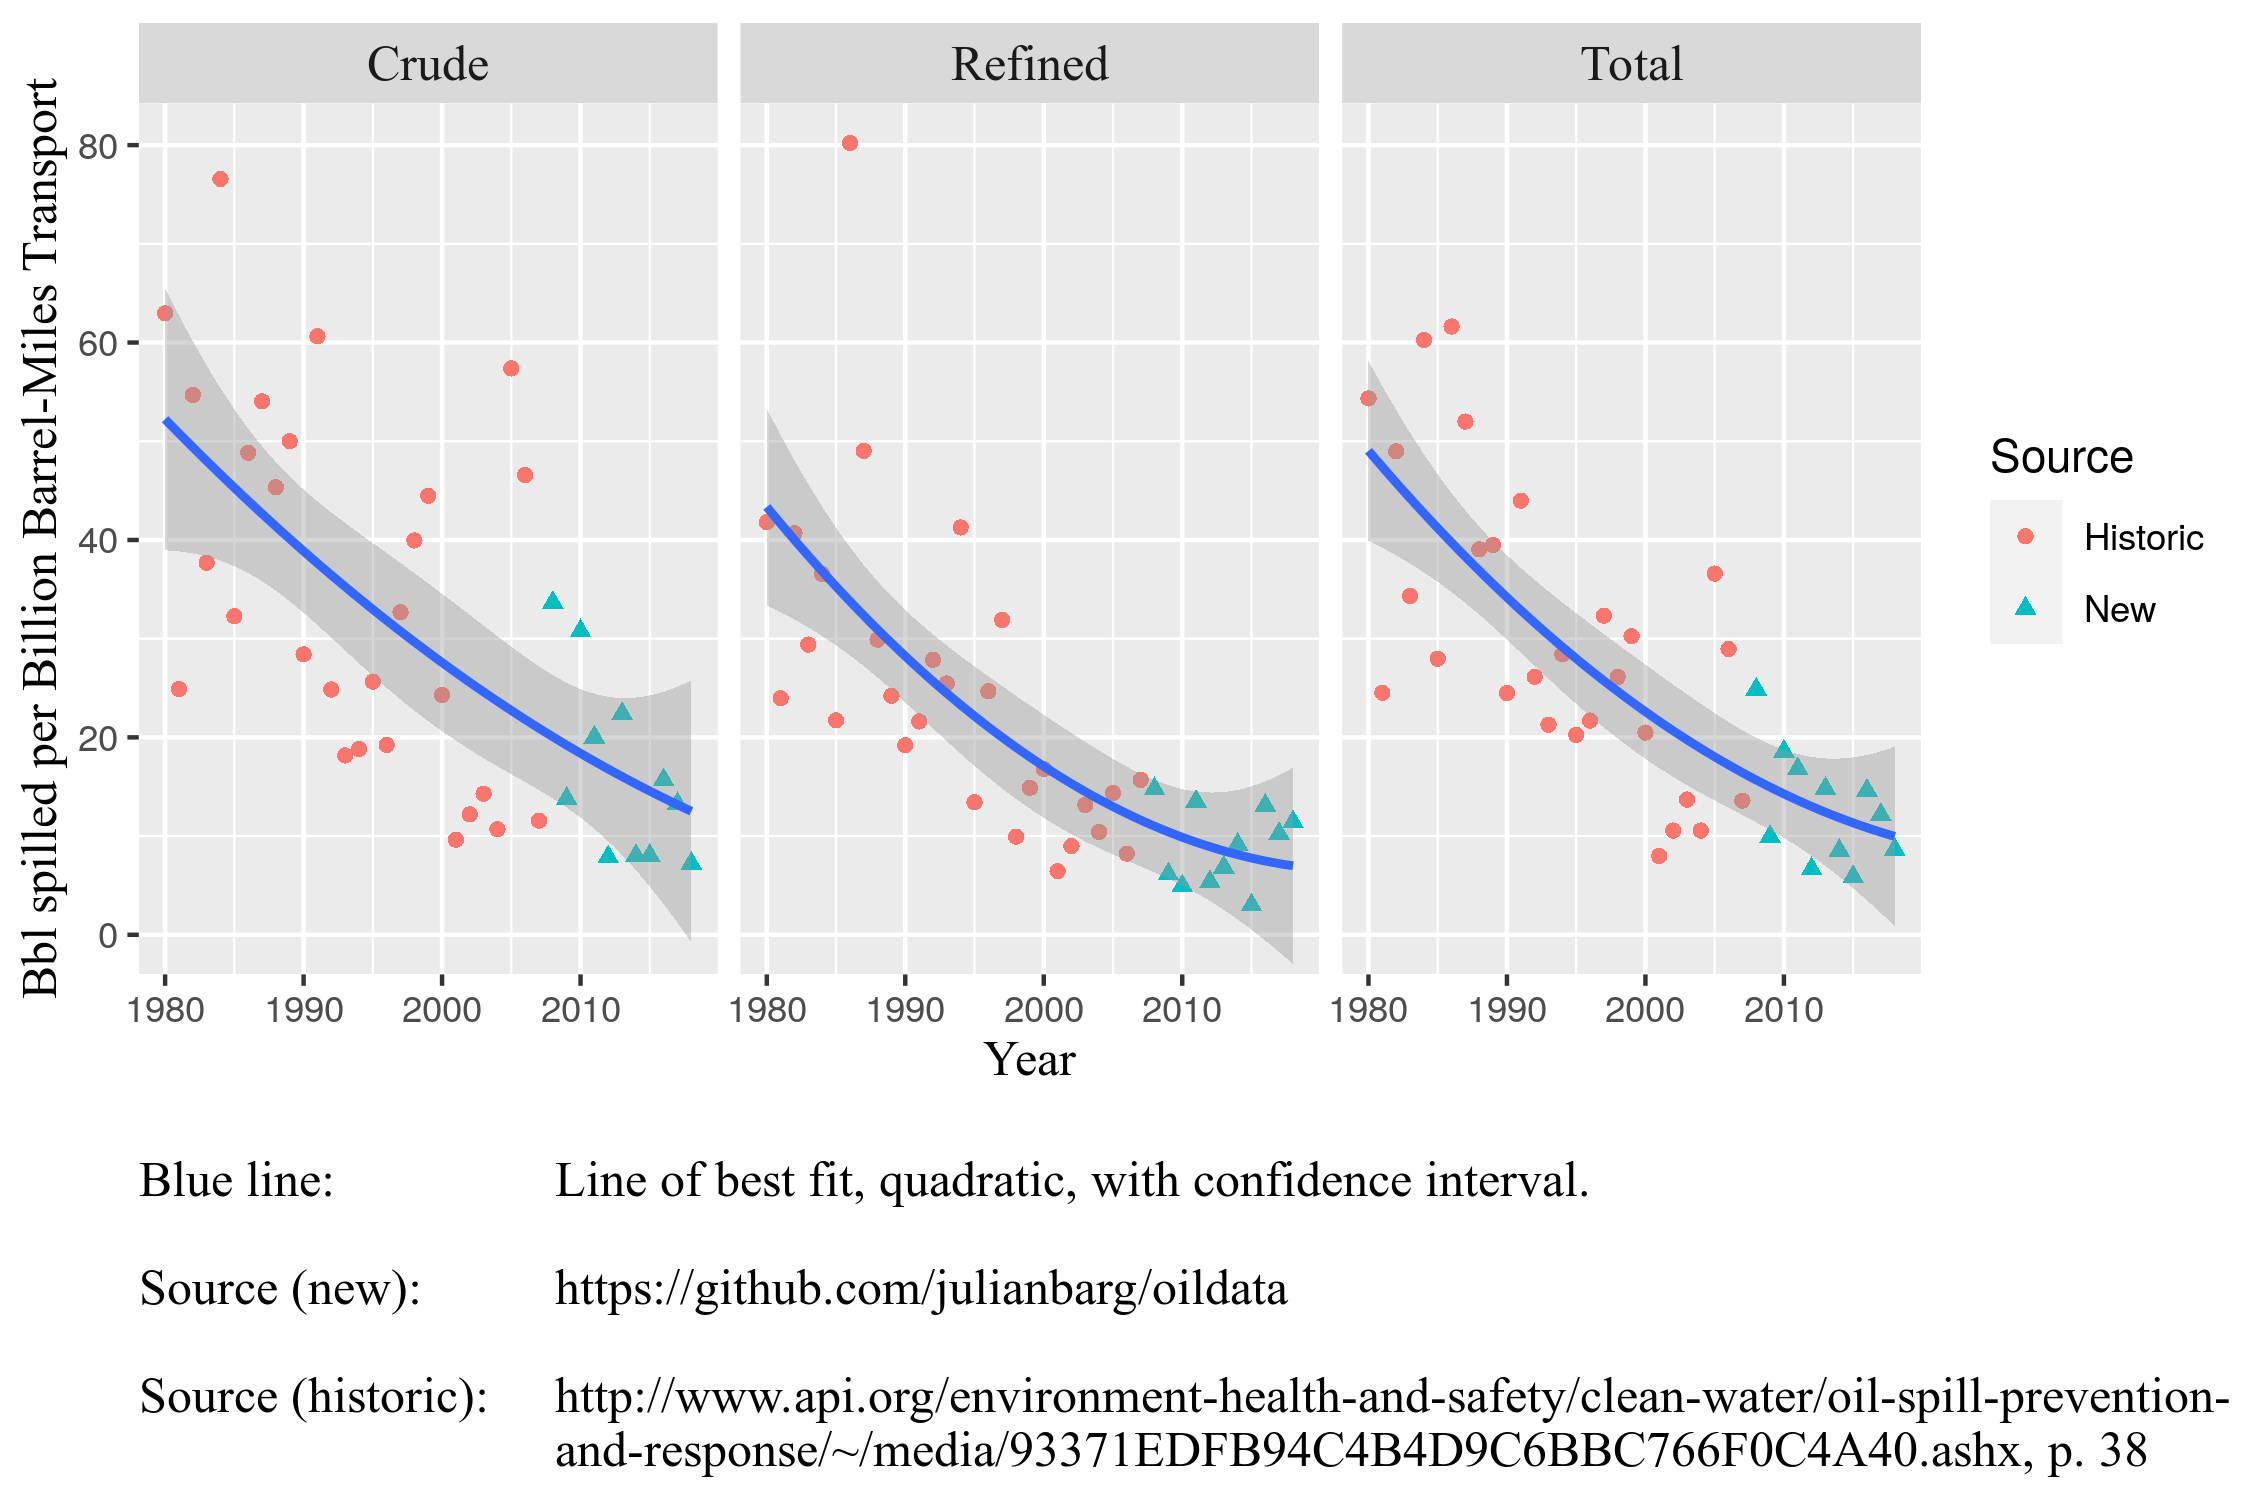
\includegraphics{../illustrations/population_learning_4.png}}
\end{figure}

An alternative view of organizational learning suggests that organizations can break out of existing trajectories and escape their constraints through learning--but that to do so requires a considerable rethinking of existing paradigms \citep{March2010}. For instance, an organization can reimagine how it measures performance \citep{Argyris1978}. This is consistent with the \textit{organizational routines} view, which holds that organizations develop not knowledge but patterns of action in stable environments \citep{Bingham2011}. The organizational routines view also postulates that in the absence of significant interventions, intricate but ultimately obsolete systems develop, for instance ones that rely on outdated technologies \citep{March1991}. With sufficient complexity, these systems can generate a never-ending stream of unexpected interactions and externalities, which then become relevant for sustainability research when the organization or industry has a catastrophic potential \citep{Perrow1984, Beck1992}. One would hope for stakeholders to be able to identify the pattern of unexpected interactions and externalities, but under an inadequate environmental regime the organization or industry can escape scrutiny through greenwashing \citep{Lyon2015}. The actions of industry level actors such as the American Petroleum Institute (API) aim as much (or more) at appeasing the public as they aim at making pipelines safer. As a result, it is difficult for us as observers to tease apart whether industry-developed technologies improve pipeline safety or serve to give the industry a safe, high-tech image.

The inconsistent predictions of the two views, and their implications for persistent environmental pollution allows us to address the this research questions from two different angles: \textit{"Why, despite the continuous efforts to develop new technology, has the safety record of the pipeline industry stagnated?"}

The first chapter analyzes the efforts of the industry from a greenwashing angle. This chapter brings to the fore the efforts of the pipeline industry to use technology as a rhetorical device. Actors across the industry have achieved a high degree of coordination and a shared understanding of the new technologies that are employed by the industry. This state of different actors holding a shared understanding is referred to in chapter three as \textit{high reliability}. Importantly, the knowledge developed by the industry does not translate into falling pipeline spill metrics. Some environmental grassroot organizations have taken notice of the trend of continuing pipeline spills, but overall the industry has been able to maintain a great degree of support from stakeholders and is able to expand its physical footprint across the country. The first chapter covers the technology-based greenwashing efforts that individual organizations and the industry undertake to keep being able to expand, and to preempt calls for substantive action.

The second chapter takes as a starting point past pipeline spills and demonstrates how pipeline operators respond to failure events, which unambiguously bring into focus opportunities for learning and improvement \citep{Madsen2010}. The chapter contrasts the learning that takes place after pipeline spills with the overall convergence of safety metrics. This divergence is explained through quantitative methods. The industry supports an organizational routines over an organizational knowledge view. The safety record has stagnated not because no new knowledge is gained, or knowledge disappears at the same rate as it is produced \citep{Argote2013-3}, as the organizational knowledge view would suggest. The organizational routines view makes no such prediction. Rather, we see as the organizational routines view suggests increasingly intricate routines with ultimately little impact on performance \citep{March1991}. This state would be described in the language of chapter three as \textit{low validity}.

The third chapter takes the findings of the second chapter and asks what conditions would allow for learning in the pipeline industry to be effective. The third chapter turns to the theory on organizational learning in search of an answer. The \textit{organizational routines} literature holds that organizations can break out of a state of convergence through what that literature calls either double-loop learning \citep{Argyris1978} or high-intellect learning \citep{March2010}. Two overlooked attributes of knowledge, \textit{validity} and \textit{reliability} could mend the split between the two streams of the organizational learning literature. \textit{Validity} describes whether knowledge does allow an organization to better understand, predict, and control problems, such as technological limitations or bottlenecks. \textit{Reliability} describes the degree to which member of the organization have command of the knowledge \citep{Rerup2020}. Validity and reliability allow for a critical view on the first question, and whether that state of convergence is inevitable. The discussion section of this dissertation shows that the recent technology development by the pipeline industry constitutes as high reliability, low validity situation.

To answer the research question, this dissertation employs data on the US pipeline industry. The pipeline industry offers an advantage over other industries with regard to studying environmental impacts, greenwashing, and learning, in that the industry's environmental pollution usubally takes place in the public. Unlike other industries, pipeline spills do not occur inside private plants, locked away from the public eye. Pipeline spills usually occur on public land that the pipeline operator has only acquired the right-of-way of. Pipeline spills also receive a lot of attention from the press, government agencies, and environmental grassroot organizations. These actors pay particular attention to large pipeline spills, which make up for a majority of annual spill volume. Finally, the scrutiny of oil spills also ensures that the reported data is more accurate. Government-employed emergency responders are on site alongside the company employees and can ensure a more accurate reporting of pollution data than is the case for routine environmental emissions.

Quantitative data from 2004-2019 allows us to observe greenwashing and learning in the pipeline industry. For this period of time, data is available from the Pipeline and Hazardous Materials Safety Administration (PHMSA) on how much oil each American operator transported over what distance every year. PHMSA also provides a dataset that contains data on each individual pipeline spill that occurred over that period of time.\footnote{See \url{https://www.phmsa.dot.gov/data-and-statistics/pipeline/source-data}, accessed 2020-08-30}. Data on the spills includes a narrative, how much oil was spilled and recovered, and what other impacts (e.g., injuries or deaths) occurred. Over the 16 years of the observation period, 6,147 pipeline spills were recorded, including 2,246 that the PHMSA classified as significant based on either a spill volume of over 50 barrels, more than \$50k in damages, or a casualty, injury, fire or explosion. Whereas crude oil pipelines period showed a significant improvement in pipeline safety over the observation period, the standardized spill volume of refined petroleum pipelines stayed as an almost constant rate of about 15bbl per billion barrel-miles transported (see Figure 1). 

As a next step, this dissertation uses text and network data to tease out greenwashing in the pipeline industry. Headquarter locations and board memberships (BoardEx) uncover connections between pipeline operators. Documents by the American Petroleum Institute (API) and the Association of Oil Pipe Lines (AOPL) reveal developments of the industry level. In addition, this research uses annual reports and safety reports to determine the strategies pursued by individual operators. Natural Language Processing (NLP)--specifically, topic modeling--reveals trends and show their diffusion through the pipeline industry. Finally, we can compare trends with the topics that emerge from the narratives on pipeline spill to distinguish substantive and non-substantive trends.

Qualitative data provides an understanding of the mechanisms of learning in the pipeline industry. The constant spill rate for refined petroleum pipelines is surprising, given the significant technological advancements in the areas of inline inspection tools, leak detection, and SCADA systems which allow for the remote supervision and control of pipelines. A repository on the largest or otherwise significant pipeline spills by the National Transportation Safety Board (NTSB) provides an in-depth understanding of accident causes. Since 1969, NTSB has authored 142 accident reports and briefs.\footnote{See \url{https://www.ntsb.gov/investigations/AccidentReports/Pages/pipeline.aspx}, accessed 2020-08-30}. For this dissertation I select the 10 most recent full accident reports. As a robustness check, I also select the 15 most significant accidents according to spill volume, net loss, number of injuries and fatalities, and property damage (top 3 per category), and collect independent archival data on these spills. As of 2020, little empirical research exists on the pipeline industry. \citet{Park2019} uses the PHMSA dataset to study how reputation affects relationships with exchange partners. \citet{Zakikhani2020} review the research into pipeline failures in the area of engineering, which has largely ignored organizational factors. More generally, oil spills are also covered by works in biology \citep[in particular][]{Burger1997} and the oil industry by works in sociology and history \citep[e.g.,][]{Dochuk2019}.

The context of pipeline spills is suitable for both questions on greenwashing and learning. Pipeline spills are periodic triggers for public debate, over the course of which organizations encounter many choice moments that could tempt them to greenwash their track record, policies, and efforts to improve pipeline safety \citep{Lyon2011}. More importantly, the American Petroleum Institute (API) and the Association of Oil Pipe Lines (AOPL) discuss pipeline safety and their communication strategy in a semi-public fashion. Pipeline spills, such as other failures, are also catalysts for learning \citep{March1991}. Learning has high visibility after large pipeline spills take place, and we can observe the learning process independent of its outcomes better than in other contexts. In summary, it is easier to obtain data on learning and greenwashing for this industry, compared to other industries, which operate far less on public lands.

Some of the findings of this dissertation might not be fully generalizable. Pipeline systems, with their manifold interactions and catastrophic potential are a great example of the complex systems and externalities discussed by \citet{Perrow1984} and citet{Beck1992}. The challenges associated with growing complexity may not be present in all other contexts. In particular, uncoupled production methods can allow for much reduced interactive potential. In these contexts, greenwashing and the convergence of performance measures might take on a different shape. The complexity of pipeline systems stems from the interaction of mechanics, physics (fluid dynamics are notoriously complicated are of physics), and complex command structures. The diverse geography and many jurisdictions of the US also add to the complexity. In addition, there is an economic incentive to run pipeline infrastructure at a very high utilization rate and throughput, e.g., by frequently changing the commodity to be transported according to demand.\footnote{Although pipelines are generally optimized for transporting specific commodities, in principle any pipeline can transport almost any commodity when demand or supply changes.} Altogether, the complexity and interactions are not far off from what \citet{Perrow1984} observed for nuclear power plants. Many other industries constitute complex systems because of their elaborate supply chain structures, a future avenue of research would thus be whether these complex supply chains bring about the same limits to learning.

I make four contributions with this research. (1) The empirical research on greenwashing highlights the potentially malevolent role that industry level organizations can play, and that technology-based claims should be taken with a grain of salt. Actors in the pipeline industry are aware of the possibility to attain a better image by creating an association between pipelines and high-tech, independent of the actual safety performance. At the same time, it is almost impossible for laymen to rebut the validity of technology that is built on decades of engineering research, and that hence the industry can safely entrench itself in this realm of modernity. Parallels may exist in other industries when technologies rather than concrete solutions to concrete problems are discussed. An example may be the use of block chain technology for the purpose of safeguarding he environment, or the use of general purpose technologies more generally, e.g., TQM \citep{Zbaracki1994}

(2) This dissertation introduces a context where organizational learning has "bottomed out" and analyzes how learning plays out under these circumstances. The context allows us to study learning despite the absence of aggregate, quantitative improvements in performance measures because (a) we can observe the process of learning independent from the outcome in qualitative data, and (b) rich data, including textual descriptions, is available on the object of learning--individual pipeline spills. This rich data allows us to distinguish a "dynamic" state where performance measures are constant because learning and emerging challenges cancel each other out from a hypothetical "state of equilibrium" where there is no new knowledge to be obtained. Thus, this dissertation brings to the fore a state that large swaths of the learning literature have taken for granted and failed to analyze: the "end of learning" period where performance measures make it appear as if the organization or industry has come to a standstill. For the pipeline industry and similar industries that constitute complex systems with catastrophic potential, the predominance of such a state over the whole extent of the learning curve and in perpetuity would be a concerning finding. The convergence of learning hypothesis suggests that stakeholders should not pin their hopes on conventional learning (in a learning curve sense) but rather push for learning that questions commonly held assumptions, as described in chapter 3.

(3) This dissertation also makes a contribution to the discourse regarding environmental sustainability and technology. The sustainability research community is split as to the role of technology for sustainability. Some work leans more toward a technocentric view with little to no consideration of social systems, for instance in research on low-carbon electricity \citep[e.g.,][]{Greenblatt2017}. Other authors emphasize the need for changes to the political and economic system in order reduce damages to the planet, such as the degrowth discourse \citep{Kallis2018}. With regard to that debate, the findings of this research highlight the role that system complexity and unexpected externalities play for continued pollution. The pipeline industry provides a very vivid example of the limits to depolluting existing technology. Further, the greenwashing in the pipeline industry that this research surfaces should act as a cautionary tale on the role and purpose of technology in communication.

(4) This dissertation moves forward theory on learning by highlighting the considerable effort necessary to leave an existing trajectory. New knowledge needs to be created that is both valid and reliable, which requires for an organization or industry to collectively question preexisting fundamental assumptions. Applied to pipeline spills, this would imply that if society was to collectively decide that oil spills at the current level are not acceptable, then we should not rely on the industry to develop technology and make changes in the current fashion. A more fundamental rethinking of the (physical and political) system of energy delivery would be necessary.

%The empirical sections of this dissertation use data from the US pipeline industry. Compared to other industries, both environmental pollution events and the subsequent learning process play out in a very public fashion in the pipeline industry. Large spills, which make up for a big share of the overall spill volume, are often discovered by members of the public, covered by the press, and investigated by independent government agencies. The context offers two advantages over existing empirical research. First, in the pipeline industry we can disentangle learning and the outcomes thereof. Empirical research on organizational learning commonly has to rely on improvements in performance variables to gauge learning \citep{Argote2011}. As in the context of the pipeline industry learning can be observed directly, the risk of an outcome bias is reduced \citep{Dillon2008}. The context also allows us to disentangle effective learning and rhetorics or greenwashing. In the pipeline industry, it is possible to determine when new technology and other measures are a response to existing problems, and when they are ineffective or even misleading talking points that serve to greenwash. The latter, in this specific context, is tied to industry level organizations such as the American Petroleum Institute (API) or the Association of Oil Pipe Lines (AOPL).

%This dissertation addresses two questions. (1) Can organizations that effectively learns from failures \citep{March1991} also stagnate? And (2) how does does an industry greenwash \citep{Lyon2015} this stagnation? Organization learning is observed to, after initially quick progress, converge to a certain value \citep{Argote2013-1}. In this process, organizations develop advanced, complex systems. \citet{Beck1992} and \citet{Perrow1984} suggest that unexpected interactions and externalities are intrinsic limitations of these systems. Only considerable rethinking of existing paradigms allows organizations to break out of the dead end that these complex systems can become \citep{Argyris1978, March2010, March1991}. The key to this breakout is validity and reliability of knowledge \citep{Rerup2020}. \citet{Lyon2011} suggest that instead of addressing externalities in the environmental realm, organizations may prefer to greenwash \citep{Lyon2011}. Trade associations are known to play a role in processes such as greenwashing when it occurs on a larger scale \citep{Maguire2009}.

%Between in-line inspection tools, leak detection technology, and SCADA systems that allow for the remote supervision and control of pipelines, it seems as if the pipeline industry has a technological solution to every problem thrown at it. \textit{Then why has the industry not improved its environmental performance in twenty years?} Further, if pipeline spills in the year 2020 are still common, this raises a follow-up question: \textit{How do pipeline operators regularly convince their stakeholders and the regulator that pipelines are safe}, and that they should be allowed to expand their physical footprint.

%Organizational forgetting ultimately is a routines view.